\chapter{Медленные системы}

\

Возьмём известную нам "быструю систему", и добавим ограничение на скорость конвейера: введём множество $\mathbb{V}$  допустимых скоростей $v_i$, каждая из которых является вполне конечной. Тогда необходимо помимо абстрактной площади начать учитывать и длину конвейеров. А так же необходимо начать учитывать взаимодействие ресурсов.

\

Обычно, в играх по типу Satisfactory и Factorio "скорость" конвейера измеряется не в метрических единицах $[v_i]$ = м/с, а как пропускная способность $[q_i]$ = шт/с. Но одно можно перевести в другое, если добавить плотность ёмкости конвейера $[\rho_i]$ = шт/м. $v_i \cdot \rho_i = q_i$

\

Однако это всё не меняет допустимый набор действий, а просто накладывает на него некоторые ограничения, и меняет суть задачи: мы перераспределяем не просто ресурсы, а пропускные способности.

$$
\left[
\begin{matrix}
	m_{11} & \ldots & m_{1n} \\
	\vdots & \ddots & \vdots \\
	m_{k1} & \ldots & m_{kn}
\end{matrix}
\right]
\times
\left[
\begin{matrix}
	q^{\text{in}}_1 \\
	\vdots \\
	q^{\text{in}}_n
\end{matrix}
\right]
=
\left[
\begin{matrix}
	q^{\text{out}}_1 \\
	\vdots \\
	q^{\text{out}}_n
\end{matrix}
\right]
$$

\

В матричной форме преобразования, элементы самой матрицы -- скаляры, а элементы векторов -- пропускные способности $[q_i]$ = шт/с

\

Важно отметить, что пропускная способность \underline{конвейера} $q_i$ и пропускная способность \underline{русурсов} $q^{\text{res}}$ -- это две разные, но взаимосвязные вещи: $q^{\text{res}}$ -- это то, что производят заводы, и что "выливается" на конвейеры, которые двигаются с $v_i$, и имеют $\rho_i$. Для адекватной работы такой системы необходимо, чтобы $q^{\text{res}} \le q_i$. В противном случае завод не сможет выкладывать ресурсы на конвейер -- то есть будет простаивать. Таким образом, схемы необходимо проектироавть с учётом этих двух величин.

\

Если же $q^{\text{res}} > q_i$ -- то возможны 2 принципиальные ситуации: $q_i = 0$ и $q_i \ne 0$. Рассмотрим первую на двух примерах:



\vspace{0.5in}

\begin{minipage}{0.5\textwidth}
	\begin{tikzpicture}[
		s/.style = {rectangle, draw=blue!60,	fill=blue!5,	very thick, minimum size=20},
		a/.style = {rectangle, draw=red!60,		fill=red!5,		very thick, minimum size=20},
		o/.style = {rectangle, draw=green!60,	fill=green!5,	very thick, minimum size=20},
		r/.style = {->, thick, rounded corners=10pt},
		]
		
		% === === Nodes === ===
		\node[o]	(in)	at	(0, 2)	{in};
		\node[s]	(s)		at	(0, 0)	{s};
		\node[o]	(out2)	at	(0, -2)	{out};
		\node[o]	(out3)	at	(2, -2)	{out};
		\node[
			regular polygon, regular polygon sides=6, 
			draw, draw=red!60, fill=red!40, 
			very thick, minimum size=1cm
			] (out1) at (-2, -2) {};
		\draw[
			rounded corners=1.25pt,
			draw, draw=white!100, fill=white!100
			] (-2.25, -2.1) rectangle (-1.75, -1.9);
		
		
		
		% === === Lines === ===
		\draw[r]	(in.south)	to	node[right]	{$q$}	(s.north);
		\draw[r]	(s.west)	-|	node[above]	{$0$}	(out1.north);
		\draw[r]	(s.south)	to	node[right]	{$q/2$}	(out2.north);
		\draw[r]	(s.east)	-|	node[above]	{$q/2$}	(out3.north);
		
	\end{tikzpicture}
\end{minipage}
\begin{minipage}{0.5\textwidth}
	\begin{tikzpicture}[
			s/.style = {rectangle, draw=blue!60,	fill=blue!5,	very thick, minimum size=20},
			a/.style = {rectangle, draw=red!60,		fill=red!5,		very thick, minimum size=20},
			o/.style = {rectangle, draw=green!60,	fill=green!5,	very thick, minimum size=20},
			r/.style = {->, thick, rounded corners=10pt},
			]
			
			% === === Nodes === ===
			\node[o]	(in)	at	(0, 4)		{in};
			\node[s]	(s1)	at	(0, 2)		{s};
			\node[s]	(s2)	at	(-2, 0)		{s};
			\node[s]	(s3)	at	(2, 0)		{s};
			\node[o]	(out2)	at	(-1, -2)	{out};
			
			\node[
				regular polygon, regular polygon sides=6, 
				draw, draw=red!60, fill=red!40, 
				very thick, minimum size=1cm
				] (out1) at (-3, -2) {};
			\draw[
				rounded corners=1.25pt,
				draw, draw=white!100, fill=white!100
				] (-3.25, -2.1) rectangle (-2.75, -1.9);
			
			\node[o]	(out3)	at	(1, -2)	{out};
			\node[o]	(out4)	at	(3, -2)	{out};
			
			
			
			
			% === === Lines === ===
			\draw[r]	(in.south)	to	node[right]	{$q$}	(s1.north);
			\draw[r]	(s1.west)	-|	node[above]	{$q/2$}	(s2.north);
			\draw[r]	(s1.east)	-|	node[above]	{$q/2$}	(s3.north);
			\draw[r]	(s2.west)	-|	node[above]	{$0$}	(out1.north);
			\draw[r]	(s2.east)	-|	node[above]	{$q/2$}	(out2.north);
			\draw[r]	(s3.west)	-|	node[above]	{$q/4$}	(out3.north);
			\draw[r]	(s3.east)	-|	node[above]	{$q/4$}	(out4.north);
		
	\end{tikzpicture}
\end{minipage}






\vspace{0.5in}

Если все конвейеры (кроме тупикового) способны полностью перевозить поданные ресурсы, а спиттеры работают мгновенно -- то сплиттер, подключённый к тупиковой ветке просто уменьшает период своей циклической группы на 1: 

$$C[t_i] \xrightarrow{\text{deadend}} C[t_i-1]$$

\

Таким образом тупик можно интерпретировать, как конвейерный разделитель с нулевым количеством выходов, а следовательно, он -- пустая циклическая группа $C[0]$.

\

Однако важно понимать, что уменьшается период лишь одного сплиттера, а не всей системы целиком, что отлично видно на второй схеме.

\

Благодоря тупиковым ветвям, можно получить преобразование: $\mathbb{T} \to \{ 2, 3 \ldots, \text{max}(\mathbb{T}) \}$, что упрощает построение многих схем.






\vspace{0.25in}

\noindent Рассмотрим теперь вторую ситуацию: $q^{\text{res}} > q_i$:

\vspace{0.5in}

\begin{tikzpicture}[
	s/.style = {rectangle, draw=blue!60,	fill=blue!5,	very thick, minimum size=20},
	a/.style = {rectangle, draw=red!60,		fill=red!5,		very thick, minimum size=20},
	o/.style = {rectangle, draw=green!60,	fill=green!5,	very thick, minimum size=20},
	r/.style = {->, thick, rounded corners=10pt},
	r2/.style = {line width=1pt, 
		double distance=1pt, 
		arrows = {-Stealth[inset=0pt, angle=45:10pt]},
		rounded corners=10pt,
		red
	},
	]
	
	% === === Nodes === ===
	\node[o]	(in)	at	(0, 2)		{in};
	\node[s]	(s)		at	(0, 0)		{s};
	\node[o]	(out1)	at	(-1, -2)	{out};
	\node[o]	(out2)	at	(1, -2)		{out};
	
	\draw[fill=black, thick] (-2,4) circle (3pt) node[right] {$\ q_0>>q$};
	\draw[fill=white, draw=red, thick] (-2,3) circle (3pt) node[right] {$\ q_1 < q/2$};
	
	
	
	% === === Lines === ===
	\draw[r]	(in.south)	to	node[right]	{$q$}	(s.north);
	\draw[r2]	(s.west)	-|	node[above]	{$q_1$}	(out1.north);
	\draw[r]	(s.east)	-|	node[above]	{$q-q_1$}	(out2.north);
	
\end{tikzpicture}



\vspace{0.5in}

Работает данная схема так: если $q_1 \ge q/2$ -- то разделитель работает по обычным правилам. В противном же случае появляется новое правило: разделитель первый цикл работает как $C[t_i]$ вплоть до посещения "критического" выхода. Как только до него доходят -- запускается таймер на $1/q_1$, и пока он не истечёт -- считается, что на этом выходе -- тупик - то есть $C[t_i] \to C[t_i-1]$

\

\noindent Иллюстрация того, \textbf{насколько} сильно может измениться суть схемы, если поставить другой конвейер:




\vspace{0.5in}

\begin{minipage}{0.5\textwidth}
	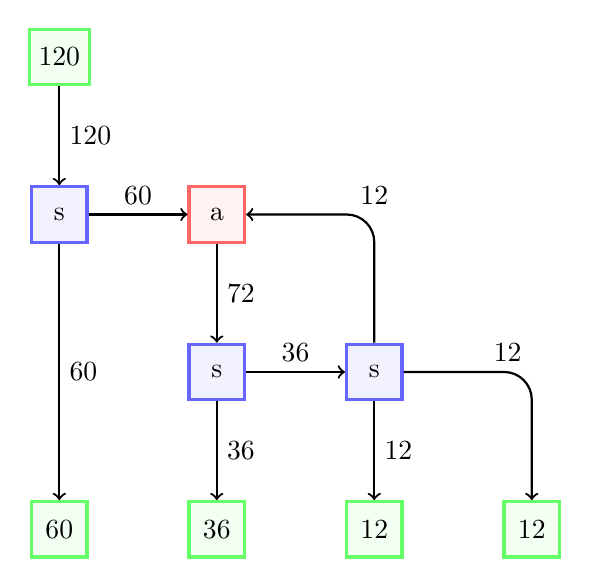
\begin{tikzpicture}[
		s/.style = {rectangle, draw=blue!60,	fill=blue!5,	very thick, minimum size=20},
		a/.style = {rectangle, draw=red!60,		fill=red!5,		very thick, minimum size=20},
		o/.style = {rectangle, draw=green!60,	fill=green!5,	very thick, minimum size=20},
		r/.style = {->, thick, rounded corners=10pt}
		]
		
		
		% === === Nodes === ===
		\node[o]	(in)	at	(0, 4)		{$120$};
		\node[s]	(s)		at	(0, 2)		{s};
		\node[a]	(a)		at	(2, 2)		{a};
		\node[s]	(s1)	at	(2, 0)		{s};
		\node[s]	(s2)	at	(4, 0)		{s};
		\node[o]	(out1)	at	(0, -2)		{$60$};
		\node[o]	(out2)	at	(2, -2)		{$36$};
		\node[o]	(out3)	at	(4, -2)		{$12$};
		\node[o]	(out4)	at	(6, -2)		{$12$};
		
		
		% === === Lines === ===
		\draw[r]	(in.south)	to	node[right]	{$120$}	(s.north);
		\draw[r]	(s.south)	to	node[right]	{$60$}	(out1.north);
		\draw[r]	(s.east)	to	node[above]	{$60$}	(a.west);
		\draw[r]	(a.south)	to	node[right]	{$72$}	(s1.north);
		\draw[r]	(s1.south)	to	node[right]	{$36$}	(out2.north);
		\draw[r]	(s1.east)	to	node[above]	{$36$}	(s2.west);
		\draw[r]	(s2.north)	|-	node[above]	{$12$}	(a.east);
		\draw[r]	(s2.south)	to	node[right]	{$12$}	(out3.north);
		\draw[r]	(s2.east)	-|	node[above left]	{$12$}	(out4.north);
		
		
	\end{tikzpicture}
\end{minipage}
\begin{minipage}{0.5\textwidth}
	\begin{tikzpicture}[
		s/.style = {rectangle, draw=blue!60,	fill=blue!5,	very thick, minimum size=20},
		a/.style = {rectangle, draw=red!60,		fill=red!5,		very thick, minimum size=20},
		o/.style = {rectangle, draw=green!60,	fill=green!5,	very thick, minimum size=20},
		r/.style = {->, thick, rounded corners=10pt},
		r2/.style = {
			line width=1pt, 
			double distance=1pt, 
			arrows = {-Stealth[inset=0pt, angle=45:10pt]},
			rounded corners=10pt,
			red
		},
		]
		
		
		% === === Nodes === ===
		\node[o]	(in)	at	(0, 4)		{$120$};
		\node[s]	(s)		at	(0, 2)		{s};
		\node[a]	(a)		at	(2, 2)		{a};
		\node[s]	(s1)	at	(2, 0)		{s};
		\node[s]	(s2)	at	(4, 0)		{s};
		\node[o]	(out1)	at	(0, -2)		{$70$};
		\node[o]	(out2)	at	(2, -2)		{$30$};
		\node[o]	(out3)	at	(4, -2)		{$10$};
		\node[o]	(out4)	at	(6, -2)		{$10$};
		
		
		% === === Lines === ===
		\draw[r]	(in.south)	to	node[right]	{$120$}	(s.north);
		\draw[r]	(s.south)	to	node[right]	{$70$}	(out1.north);
		\draw[r]	(s.east)	to	node[above]	{$50$}	(a.west);
		\draw[r2]	(a.south)	to	node[right]	{$60$}	(s1.north);
		\draw[r]	(s1.south)	to	node[right]	{$30$}	(out2.north);
		\draw[r]	(s1.east)	to	node[above]	{$30$}	(s2.west);
		\draw[r]	(s2.north)	|-	node[above]	{$10$}	(a.east);
		\draw[r]	(s2.south)	to	node[right]	{$10$}	(out3.north);
		\draw[r]	(s2.east)	-|	node[above left]	{$10$}	(out4.north);
		
		
	\end{tikzpicture}
\end{minipage}





\vspace{0.5in}

Как видим, такая разница происходит из-за того, что ограниченный конвейер подключенн на выход соединителя. Он превращается в тупик по тем же принципам, что и у сплиттера.

\

Однако сдесь у нас 2 \textbf{взаимосвязанных} конвейера заходят в "бутылочное горлышко", так что скорость основного из них стабилизируется, как единственное решение уравнения

\begin{align*}
	&q_0 \cdot \left( 1 - \frac16 \right) = 60 \\
	&q_0 \cdot \frac65 = 60 \\
	&q_0 = 50
\end{align*}


\

Но тут у нас \textbf{единственное} решение -- а если их несколько? рассмотрим пример, в котором у нас несколько \textbf{независимых} входов:




\vspace{0.5in}

\begin{tikzpicture}[
	s/.style = {rectangle, draw=blue!60,	fill=blue!5,	very thick, minimum size=20},
	a/.style = {rectangle, draw=red!60,		fill=red!5,		very thick, minimum size=20},
	o/.style = {rectangle, draw=green!60,	fill=green!5,	very thick, minimum size=20},
	r/.style = {->, thick, rounded corners=10pt},
	r2/.style = {
		line width=1pt, 
		double distance=1pt, 
		arrows = {-Stealth[inset=0pt, angle=45:10pt]},
		rounded corners=10pt,
		red
	},
	]
	
	\draw[fill=black, thick] (-2,5) circle (3pt) node[right] {$\ q>>q_1, q_2$};
	\draw[fill=white, draw=red, thick] (-2,4) circle (3pt) node[right] {$\ q_0 < s_1/2+q_2/2$};
	
	
	% === === Nodes === ===
	\node[o]	(in1)	at	(-2, 2)		{$q_1$};
	\node[o]	(in2)	at	(2, 2)		{$q_2$};
	\node[s]	(s1)	at	(-2, 0)		{s};
	\node[s]	(s2)	at	(2, 0)		{s};
	\node[a]	(a)		at	(0, 0)		{a};
	\node[o]	(out1)	at	(-2, -2)	{$q_1-x$};
	\node[o]	(out2)	at	(0, -2)		{$q_0$};
	\node[o]	(out3)	at	(2, -2)		{$q_2-y$};
	
	
	% === === Lines === ===
	\draw[r]	(in1.south)	to	node[right]	{$q_1$}		(s1.north);
	\draw[r]	(in2.south)	to	node[right]	{$q_2$}		(s2.north);
	\draw[r]	(s1.south)	to	node[right]	{$q_1-x$}	(out1.north);
	\draw[r]	(s2.south)	to	node[right]	{$q_2-x$}	(out3.north);
	\draw[r]	(s1.east)	to	node[above]	{$x$}		(a.west);
	\draw[r]	(s2.west)	to	node[above]	{$y$}		(a.east);
	\draw[r2]	(a.south)	to	node[right]	{$x+y$}		(out2.north);
	
	
\end{tikzpicture}






\vspace{0.5in}

Очень сильно хочется сказать "пускай $x=y$" -- тогда $x = \frac{q_0}2$. Но на деле нам ничто не гарантирует такого: на деле соединитель может приоритезировать один из входов. Второй случай более интересный: например, в satisfactory есть отдельный тип соеденителя -- приоритетный соединитель (англ: priority merger), в котором есть переключатели степени приоритетности того или иного входа.

\

\noindent Пускай левый вход имеет бóльший приоритет. Рассмотрим возможные ситуации:

\begin{itemize}
	\item $\frac{q_1}2 \le q_0$: $x = \frac{q_1}2$, $y = q_0 - \frac{q_1}2$
	
	\item $\frac{q_1}2 \ge q_0$: $x = q_0$, $y = 0$
\end{itemize}






\vspace{0.5in}

\begin{minipage}{0.333\textwidth}
	\begin{tikzpicture}[
		s/.style = {rectangle, draw=blue!60,	fill=blue!5,	very thick, minimum size=15},
		a/.style = {rectangle, draw=red!60,		fill=red!5,		very thick, minimum size=15},
		o/.style = {rectangle, draw=green!60,	fill=green!5,	very thick, minimum size=15},
		r/.style = {->, thick, rounded corners=7.5pt},
		r2/.style = {
			line width=1pt, 
			double distance=1pt, 
			arrows = {-Stealth[inset=0pt, angle=45:10pt]},
			rounded corners=7.5pt,
			red
			},
		]
		
		
		% === === Nodes === ===
		\node[o]	(in1)	at	(-1.5, 1.5)		{$100$};
		\node[o]	(in2)	at	(1.5, 1.5)		{$140$};
		\node[s]	(s1)	at	(-1.5, 0)		{s};
		\node[s]	(s2)	at	(1.5, 0)		{s};
		\node[a]	(a)		at	(0, 0)			{a};
		\node[o]	(out1)	at	(-1.5, -1.5)	{$70$};
		\node[o]	(out2)	at	(0, -1.5)		{$60$};
		\node[o]	(out3)	at	(1.5, -1.5)		{$110$};
		
		
		% === === Lines === ===
		\draw[r]	(in1.south)	to	node[right]	{$100$}		(s1.north);
		\draw[r]	(in2.south)	to	node[right]	{$140$}		(s2.north);
		\draw[r]	(s1.south)	to	node[right]	{$70$}		(out1.north);
		\draw[r]	(s2.south)	to	node[right]	{$110$}		(out3.north);
		\draw[r]	(s1.east)	to	node[above]	{$30$}		(a.west);
		\draw[r]	(s2.west)	to	node[above]	{$30$}		(a.east);
		\draw[r2]	(a.south)	to	node[right]	{$60$}		(out2.north);
		
		
	\end{tikzpicture}
\end{minipage}
\begin{minipage}{0.333\textwidth}
	\begin{tikzpicture}[
		s/.style = {rectangle, draw=blue!60,	fill=blue!5,	very thick, minimum size=15},
		a/.style = {rectangle, draw=red!60,		fill=red!5,		very thick, minimum size=15},
		o/.style = {rectangle, draw=green!60,	fill=green!5,	very thick, minimum size=15},
		r/.style = {->, thick, rounded corners=7.5pt},
		r2/.style = {
			line width=1pt, 
			double distance=1pt, 
			arrows = {-Stealth[inset=0pt, angle=45:10pt]},
			rounded corners=7.5pt,
			red
			},
		]
		
		
		% === === Nodes === ===
		\node[o]	(in1)	at	(-1.5, 1.5)		{$100$};
		\node[o]	(in2)	at	(1.5, 1.5)		{$140$};
		\node[s]	(s1)	at	(-1.5, 0)		{s};
		\node[s]	(s2)	at	(1.5, 0)		{s};
		
		\node[
			draw=red!60, fill=red!5, very thick,
			regular polygon, regular polygon sides=3, 
			rotate=-90, minimum size=0.2cm
			] 
			(tri) at (-0.3, 0) {};
		\node[a]	(a)		at	(0, 0)			{p};
		\node				at	(-0.35, 0)		{$1$};
		
		\node[o]	(out1)	at	(-1.5, -1.5)	{$50$};
		\node[o]	(out2)	at	(0, -1.5)		{$60$};
		\node[o]	(out3)	at	(1.5, -1.5)		{$130$};
		
		
		% === === Lines === ===
		\draw[r]	(in1.south)	to	node[right]	{$100$}		(s1.north);
		\draw[r]	(in2.south)	to	node[right]	{$140$}		(s2.north);
		\draw[r]	(s1.south)	to	node[right]	{$50$}		(out1.north);
		\draw[r]	(s2.south)	to	node[right]	{$130$}		(out3.north);
		\draw[r]	(s1.east)	to	node[above]	{$50$}		(tri.south);
		\draw[r]	(s2.west)	to	node[above]	{$10$}		(a.east);
		\draw[r2]	(a.south)	to	node[right]	{$60$}		(out2.north);
		
		
	\end{tikzpicture}
\end{minipage}
\begin{minipage}{0.333\textwidth}
	\begin{tikzpicture}[
		s/.style = {rectangle, draw=blue!60,	fill=blue!5,	very thick, minimum size=15},
		a/.style = {rectangle, draw=red!60,		fill=red!5,		very thick, minimum size=15},
		o/.style = {rectangle, draw=green!60,	fill=green!5,	very thick, minimum size=15},
		r/.style = {->, thick, rounded corners=7.5pt},
		r2/.style = {
			line width=1pt, 
			double distance=1pt, 
			arrows = {-Stealth[inset=0pt, angle=45:10pt]},
			rounded corners=7.5pt,
			red
			},
		]
		
		
		% === === Nodes === ===
		\node[o]	(in1)	at	(-1.5, 1.5)		{$100$};
		\node[o]	(in2)	at	(1.5, 1.5)		{$140$};
		\node[s]	(s1)	at	(-1.5, 0)		{s};
		\node[s]	(s2)	at	(1.5, 0)		{s};
		
		\node[
			draw=red!60, fill=red!5, very thick,
			regular polygon, regular polygon sides=3, 
			rotate=-90, minimum size=0.2cm
			] 
			(tri) at (-0.3, 0) {};
		\node[a]	(a)		at	(0, 0)			{p};
		\node				at	(-0.35, 0)		{$1$};
		
		\node[o]	(out1)	at	(-1.5, -1.5)	{$70$};
		\node[o]	(out2)	at	(0, -1.5)		{$30$};
		\node[o]	(out3)	at	(1.5, -1.5)		{$140$};
		
		
		
		% === === Lines === ===
		\draw[r]	(in1.south)	to	node[right]	{$100$}		(s1.north);
		\draw[r]	(in2.south)	to	node[right]	{$140$}		(s2.north);
		\draw[r]	(s1.south)	to	node[right]	{$70$}		(out1.north);
		\draw[r]	(s2.south)	to	node[right]	{$140$}		(out3.north);
		\draw[r]	(s1.east)	to	node[above]	{$30$}		(tri.south);
		\draw[r]	(s2.west)	to	node[above]	{$0$}		(a.east);
		\draw[r2]	(a.south)	to	node[right]	{$30$}		(out2.north);
		
		
	\end{tikzpicture}
\end{minipage}






\vspace{0.5in}

Таким образом приоритетный соединитель работает по следующему алгоритму: когда во вход приходит первый ресурс-- он сразу выходит на конвейер $q$. После этого запускается таймер на $1/q$, на протяжении которого никакие ресурсы не выходят, а просто выстраиваютсяв приоритетную очередь. Когда таймер кончается -- ресурс с бóльшим приоритетом выходит, и заново запускается таймер.

\

При этом так же можно добавить приорететный соединитель, который пускает ресурсы только в рамках заданного соотношения $x:y$ по следующему принципу: выходная скорость $q$ делится на $x+y$. если суммарно с левого $q_1$ и правого $q_2$ входа приходит не больше, чем $q$ -- то

































































































































